\section{Dynamic Diagrams}
A dynamic diagram contains a set of a scenario descriptions, object groups, object stacks, objects, and message relations. In this section, the representation (in the context) and checking these will be explained

The dynamic object representation in the context is rooted in a deferred \textsc{tbon$\_$tc$\_$dynamic$\_$object} class. All known dynamic diagram components are subtypes of this class. Not all the aforementioned kinds of dynamic diagrams are represented directly by a class in the context though. Since an object and an object\_stack are syntactically equal, except for the keyword itself, they do not need separate representations \cite[p. 358]{walden1995}. However, they are both represented by the \textsc{tbon$\_$tc$\_$object} class. Lastly, message relations are not represented in a designated object, since they only consists of dynamic references. With this simple structure of message relations, checking them only require checking the dynamic references, and as such a dedicated object for this element is unnecessary. Scenario description and object group are both represented directly as they appear in the grammar.

\begin{figure}[h]
\centerline{
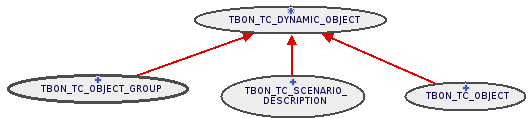
\includegraphics[scale=0.7]{images/dynamic-diagram.png}
}
\caption{Inheritance structure for dynamic diagrams.}
\label{fig:dynamic-diagram}
\end{figure}

\paragraph{}
When checking dynamic diagrams, because of the object based nature of the diagrams, as opposed to the class based nature of the other kinds of specifications, two new contexts are introduced. The object context keeps track of the objects in a dynamic diagram. Objects mentioned by message relations must be defined by objects or object stacks. The object context is used for this. Similarly, any scenario mentioned by a message relation must be defined by a scenario description. When encountering new scenarios, the type checker adds them to the context, in which it can then check if they are present when mentioned in message relations.

\paragraph{}
Even though some elements are not represented by the a designated class in the context, they still need to be type checked as separate entities. In order for a scenario description to be well-typed, its name must be unique. Having more than one scenario with the same name would ruin the semantic value of describing a scenario. Scenarios are represented by strings, however integer ranges are supported by the type checker (as seen in\cite[pp. 379-380]{walden1995}). When parsing strings of the structure \textsc{integer} ``-" \textsc{integer}, the type checker will split up the range and create multiple scenarios, one for each number in the range. The example in figure \ref{fig:integer_range} would therefore result in nine different scenarios. Everything other than integer ranges are just parsed directly as strings. Only the scenario labels (e.g. ``1-3") are interesting for the type checker as the description of a scenario can have any value.

\begin{figure}[H]
{\footnotesize
\begin{verbatim}
 1| dynamic_diagram Start_car
 2| component
 3|    scenario "Scenario 1: Start the car"
 4|    action
 5|       "1-3"     "Put key in keyhole"
 6|       "4-5"     "Turn key"
 7|       "7-9"     "Drive"
 8|     end
 9| end
\end{verbatim}
}
\caption{Example of use of integer ranges in scenario descriptions.}
\label{fig:integer_range}
\end{figure}

Similar to scenarios, object groups must have unique names, or be nameless. Furthermore all its contained elements (dynamic components) must also be well-typed, in order for the object group to be well-typed.

Due to their similarity, objects and object stacks are checked in the same way, however not by the same feature. Had they been in the same feature it would have meant complications when expanding the system, or changing the semantics of object stack. Having separate features also gives cleaner code, as different error messages can be emitted. Well-typed objects and object stacks must have unique names.

A message relation consists of two dynamic references and a scenario, which both must be well-typed. Both dynamic references must be mentioned by an object or object stack, and as such must be in the object context. Message labels are compared directly to the content of the scenario content, and must therefore be identical with one of the action label in order to be well-typed. The example seen in \cite[p. 380]{walden1995} are therefore not considered well-typed by the type checker.

\begin{figure}[H]
{\footnotesize
\begin{verbatim}
 1| dynamic_diagram open_fridge
 2| component
 3|    scenario "Scenario 2: Open fridge"
 4|    action
 5|       "1"       "Grab handle"
 6|       "2-3"     "Pull door"
 7|       "4"       "Look at the food"
 8|     end
 9|     object FRIDGE.door_handle 
10|     object HAND
11|     object EYES
12|     object FRIDGE.content
13|     HAND calls FRIDGE.door_handle "1"
14|     HAND calls FRIDGE.door_handle "2-3"
15|     EYES calls FRIDGE.content "4: Is there any bacon?"
16| end
\end{verbatim}
}
\caption{Example a scenario chart that is not well-typed.}
\label{fig:not_well_typed}
\end{figure}

\paragraph{}
The example in figure \ref{fig:not_well_typed} is not well-typed for two reasons. In line 14 the scenario mentioned is labelled ``2-3". While this is identical to the string in line 6, the the type checker has parsed this into two different scenarios with labels ``2" and ``3". To references these labels one would therefore have to use strings ``2" and ``3" and not ``2-3". Other ways of expressing sets such as ``2, 3" or ``[2; 3]" are not parsed, and will be considered as manifest. The other reason can be found in line 15. While it is suggested by Wald\'{e}n and Nerson in \cite{walden1995} that this structure is allowed it has not been included in this implementation.